\documentclass{standalone}

\usepackage{tikz}
\usepackage[T1]{fontenc}
\usepackage[tt=false, type1=true]{libertine}
\usepackage[varqu]{zi4}
\usepackage[libertine]{newtxmath}

\usetikzlibrary{shapes, positioning, calc}

\begin{document}

{\scriptsize
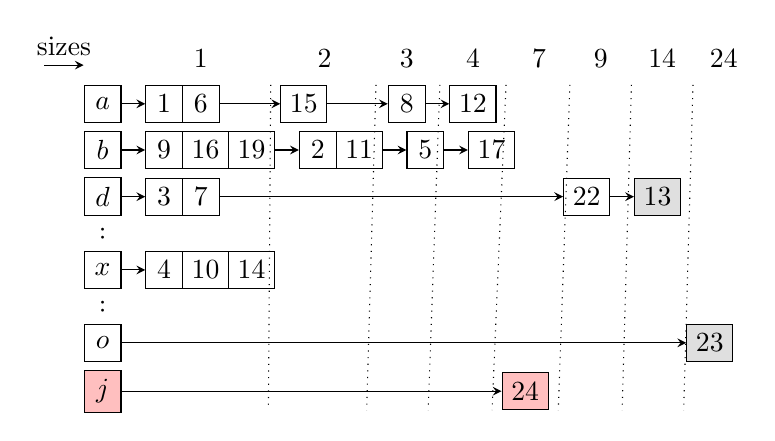
\begin{tikzpicture}
  \newcommand\listspacing{0.1}
  \newcommand\listpartspacing{0.3}
  \newcommand\arraypartspacing{0.015} % 0.03 for thick
  \newcommand\listdir{right}
  \newcommand\lbldir{below}
  %\renewcommand\ptr{$\rightarrow$}
  \newcommand\listelemminwidth{0.4675cm }
  \newcommand\listelemminheight{0.4675cm}

  \tikzset{ptr/.style={->, >=stealth}}

  % inverted lists
  \node[draw, minimum width=\listelemminwidth, minimum height=\listelemminheight] at (0, 0) (il1) {$a$};
  \foreach \label/\ilid [count=\x from 1] in {b/2, d/3}{
    \node[draw, minimum width=\listelemminwidth, minimum height=\listelemminheight, \lbldir=\listspacing of il\x] (il\ilid) {$\label$};
  }

  \node[\lbldir=0 of il3] (ilvdots-1) {\rotatebox{90}{..}};
  \node[draw, minimum width=\listelemminwidth, minimum height=\listelemminheight, \lbldir=0 of ilvdots-1] (il4) {$x$};
  \node[\lbldir=0 of il4] (ilvdots-2) {\rotatebox{90}{..}};
  \node[draw, minimum width=\listelemminwidth, minimum height=\listelemminheight, \lbldir=0 of ilvdots-2] (il5) {$o$};
  \node[draw, minimum width=\listelemminwidth, minimum height=\listelemminheight, \lbldir=\listspacing of il5, fill=red, fill opacity=0.25, text opacity=1] (il6) {$j$};

  % partition 1
  \node[draw, minimum width=\listelemminwidth, minimum height=\listelemminheight, \listdir=\listpartspacing of il1] (il1-1) {$1$};
  \foreach \poid/\idx [count=\x from 1] in {6/2}{
    \node[draw, minimum width=\listelemminwidth, minimum height=\listelemminheight, \listdir=-\arraypartspacing of il1-\x] (il1-\idx) {$\poid$};
  }
  \foreach \poid/\idx [count=\x from 2] in {/3}{
    \node[minimum width=\listelemminwidth, minimum height=\listelemminheight, \listdir=-\arraypartspacing of il1-\x] (il1-\idx) {$\poid$};
  }

  \node[draw, minimum width=\listelemminwidth, minimum height=\listelemminheight, \listdir=\listpartspacing of il2] (il2-1) {$9$};
  \foreach \poid/\idx [count=\x from 1] in {16/2, 19/3}{
    \node[draw, minimum width=\listelemminwidth, minimum height=\listelemminheight, \listdir=-\arraypartspacing of il2-\x] (il2-\idx) {$\poid$};
  }

  \node[draw, minimum width=\listelemminwidth, minimum height=\listelemminheight, \listdir=\listpartspacing of il3] (il3-1) {$3$};
  \foreach \poid/\idx [count=\x from 1] in {7/2}{
    \node[draw, minimum width=\listelemminwidth, minimum height=\listelemminheight, \listdir=-\arraypartspacing of il3-\x] (il3-\idx) {$\poid$};
  }
  \foreach \poid/\idx [count=\x from 2] in {/3}{
    \node[minimum width=\listelemminwidth, minimum height=\listelemminheight, \listdir=-\arraypartspacing of il3-\x] (il3-\idx) {$\poid$};
  }

  \node[draw, minimum width=\listelemminwidth, minimum height=\listelemminheight, \listdir=\listpartspacing of il4] (il4-1) {$4$};
  \foreach \poid/\idx [count=\x from 1] in {10/2, 14/3}{
    \node[draw, minimum width=\listelemminwidth, minimum height=\listelemminheight, \listdir=-\arraypartspacing of il4-\x] (il4-\idx) {$\poid$};
  }

  \node[minimum width=\listelemminwidth, minimum height=\listelemminheight, \listdir=\listpartspacing of il5] (il5-1) {};
  \foreach \poid/\idx [count=\x from 1] in {/2, /3}{
    \node[minimum width=\listelemminwidth, minimum height=\listelemminheight, \listdir=-\arraypartspacing of il5-\x] (il5-\idx) {$\poid$};
  }

  \node[minimum width=\listelemminwidth, minimum height=\listelemminheight, \listdir=\listpartspacing of il6] (il6-1) {};
  \foreach \poid/\idx [count=\x from 1] in {/2, /3}{
    \node[minimum width=\listelemminwidth, minimum height=\listelemminheight, \listdir=-\arraypartspacing of il6-\x] (il6-\idx) {$\poid$};
  }

  % partition 2
  \node[draw, minimum width=\listelemminwidth, minimum height=\listelemminheight, \listdir=\listpartspacing of il1-3] (il1-4) {$15$};
  \foreach \poid/\idx [count=\x from 4] in {/5}{
    \node[minimum width=\listelemminwidth, minimum height=\listelemminheight, \listdir=-\arraypartspacing of il1-\x] (il1-\idx) {$\poid$};
  }

  \node[draw, minimum width=\listelemminwidth, minimum height=\listelemminheight, \listdir=\listpartspacing of il2-3] (il2-4) {$2$};
  \foreach \poid/\idx [count=\x from 4] in {11/5}{
    \node[draw, minimum width=\listelemminwidth, minimum height=\listelemminheight, \listdir=-\arraypartspacing of il2-\x] (il2-\idx) {$\poid$};
  }

  \node[minimum width=\listelemminwidth, minimum height=\listelemminheight, \listdir=\listpartspacing of il3-3] (il3-4) {};
  \foreach \poid/\idx [count=\x from 4] in {/5}{
    \node[minimum width=\listelemminwidth, minimum height=\listelemminheight, \listdir=-\arraypartspacing of il3-\x] (il3-\idx) {$\poid$};
  }

  \node[minimum width=\listelemminwidth, minimum height=\listelemminheight, \listdir=\listpartspacing of il4-3] (il4-4) {};
  \foreach \poid/\idx [count=\x from 4] in {/5}{
    \node[minimum width=\listelemminwidth, minimum height=\listelemminheight, \listdir=-\arraypartspacing of il4-\x] (il4-\idx) {$\poid$};
  }

  \node[minimum width=\listelemminwidth, minimum height=\listelemminheight, \listdir=\listpartspacing of il5-3] (il5-4) {};
  \foreach \poid/\idx [count=\x from 4] in {/5}{
    \node[minimum width=\listelemminwidth, minimum height=\listelemminheight, \listdir=-\arraypartspacing of il5-\x] (il5-\idx) {$\poid$};
  }

  \node[minimum width=\listelemminwidth, minimum height=\listelemminheight, \listdir=\listpartspacing of il6-3] (il6-4) {};
  \foreach \poid/\idx [count=\x from 4] in {/5}{
    \node[minimum width=\listelemminwidth, minimum height=\listelemminheight, \listdir=-\arraypartspacing of il6-\x] (il6-\idx) {$\poid$};
  }

  % partition 3
  \node[draw, minimum width=\listelemminwidth, minimum height=\listelemminheight, \listdir=\listpartspacing of il1-5] (il1-6) {$8$};

  \node[draw, minimum width=\listelemminwidth, minimum height=\listelemminheight, \listdir=\listpartspacing of il2-5] (il2-6) {$5$};

  \foreach \listid in {3, 4, 5, 6}{
    \node[minimum width=\listelemminwidth, minimum height=\listelemminheight, \listdir=\listpartspacing of il\listid-5] (il\listid-6) {};
  }

  % partition 4
  \node[draw, minimum width=\listelemminwidth, minimum height=\listelemminheight, \listdir=\listpartspacing of il1-6] (il1-7) {$12$};

  \node[draw, minimum width=\listelemminwidth, minimum height=\listelemminheight, \listdir=\listpartspacing of il2-6] (il2-7) {$17$};

  \foreach \listid in {3, 4, 5, 6}{
    \node[minimum width=\listelemminwidth, minimum height=\listelemminheight, \listdir=\listpartspacing of il\listid-6] (il\listid-7) {};
  }

  % partition 5
  \foreach \listid in {1, 3, 5}{
    \node[minimum width=\listelemminwidth, minimum height=\listelemminheight, \listdir=\listpartspacing of il\listid-7] (il\listid-8) {};
  }

  \node[draw, minimum width=\listelemminwidth, minimum height=\listelemminheight, \listdir=\listpartspacing of il6-7, fill=red, fill opacity=0.25, text opacity=1] (il6-8) {$24$};

  % partition 6
  \foreach \listid in {1, 5, 6}{
    \node[minimum width=\listelemminwidth, minimum height=\listelemminheight, \listdir=\listpartspacing of il\listid-8] (il\listid-9) {};
  }

  \node[draw, minimum width=\listelemminwidth, minimum height=\listelemminheight, \listdir=\listpartspacing of il3-8] (il3-9) {$22$};

  % partition 7
  \foreach \listid in {1, 5, 6}{
    \node[minimum width=\listelemminwidth, minimum height=\listelemminheight, \listdir=\listpartspacing of il\listid-9] (il\listid-10) {};
  }

  \node[draw, minimum width=\listelemminwidth, minimum height=\listelemminheight, \listdir=\listpartspacing of il3-9, fill=gray, fill opacity=0.25, text opacity=1] (il3-10) {$13$};

  % partition 8
  \foreach \listid in {1, 6}{
    \node[minimum width=\listelemminwidth, minimum height=\listelemminheight, \listdir=\listpartspacing of il\listid-10] (il\listid-11) {};
  }

  \node[draw, minimum width=\listelemminwidth, minimum height=\listelemminheight, \listdir=\listpartspacing of il5-10, fill=gray, fill opacity=0.25, text opacity=1] (il5-11) {$23$};

  % pointers
  \foreach \listid in {1, 2, 3, 4}{
    \draw[ptr] (il\listid) -- (il\listid-1);
  }
  \draw[ptr] (il5) -- (il5-11);
  \draw[ptr] (il6) -- (il6-8);

  \draw[ptr] (il1-2) -- (il1-4);
  \draw[ptr] (il2-3) -- (il2-4);

  \draw[ptr] (il1-4) -- (il1-6);
  \draw[ptr] (il2-5) -- (il2-6);

  \draw[ptr] (il1-6) -- (il1-7);
  \draw[ptr] (il2-6) -- (il2-7);

  \draw[ptr] (il3-2) -- (il3-9);

  \draw[ptr] (il3-9) -- (il3-10);

  \draw[ptr] ($(il1.north west)+(-0.5,0.25)$) -- node[above] {sizes} ++(0.5, 0);

  % delimiters
  \foreach \a/\b in {3/4, 5/6, 6/7, 7/8, 8/9, 9/10, 10/11}{
    \draw[dotted] ($(il1-\a.north)!0.5!(il1-\b.north)$) -- ($(il6-\a.south)!0.5!(il6-\b.south)$);
  }

  % sizes
  \foreach \size/\elemid in {1/2, 3/6, 4/7, 7/8, 9/9, 14/10, 24/11}{
    \node[above=\listspacing of il1-\elemid] {$\size$};
  }
  \coordinate (il1-45mid) at ($(il1-4.north)!0.5!(il1-5.north)$);
  \node[above=\listspacing of il1-45mid] {$2$};
\end{tikzpicture}}

\end{document}
